
\chapter{بهبود الگوریتم \lr{A*}}\label{ch3}


\section{  نظریه پایه الگوریتم سنتی \lr{A*}}\label{algor}
الگوریتم \lr{َA*} یک روش جستجوی هیوریستیک\LTRfootnote{\lr{heuristic}} و بهترین-اول\LTRfootnote{\lr{best-first}} برای یافتن کم‌هزینه‌ترین مسیر است که نسبت به جستجوهای کور مزیت دارد. نکات کلیدی آن عبارتند از:

\textbf{نحوه عملکرد:} این الگوریتم با استفاده از یک جدول باز و یک جدول بسته، گره‌ها را بر اساس تابع ارزیابی زیر بررسی و انتخاب می‌کند.

\begin{equation}\label{eq1}
	f(n)=g(n)+h(n)
\end{equation}
در رابطه \eqref{eq1} جمله‌ی $ g(n) $ نمایانگر هزینه طی شده از مبدأ تا گره فعلی، $ h(n) $ تخمین هزینه از گره فعلی تا مقصد و $ f(n) $ برابر با هزینه کل ارزیابی شده برای گره است.

\textbf{مزیت اصلی:} این الگوریتم همواره گره‌ای با کمترین مقدار $ f(n) $ را انتخاب می‌کند و انعطاف‌پذیری بالایی در استفاده از انواع فاصله‌های هیوریستیک (مانند اقلیدسی یا منهتن) دارد.

شبه‌کد این الگوریتم را در صفحه‌ی بعد مشاهده می‌کنید.

\begin{latin}
	\begin{algorithm}
    \caption{$\mathsf{A}^{\!*}$ Pathfinding Algorithm}
		\label{psudo1}
		\begin{algorithmic}[1]
			\Require Start node $start$, goal node $goal$, heuristic function $h(n)$, graph with edge costs $d(u,v)$
			\Ensure Shortest path from $start$ to $goal$ as a list of nodes, or $failure$ if no path exists
			\Function{reconstruct\_path}{came\_from, current}
			\State $total\_path \gets \{current\}$
			\While{$current in came\_from.keys$}
			\State $current \gets came\_from[current]$
			\State $total\_path.prepend(current)$
			\EndWhile
			\State \Return $total\_path$
			\EndFunction
			
			\Function{a\_star}{start, goal, h}
			\State $open\_set \gets \{start\}$
			\State $came\_from \gets \text{empty map}$
			\State $g\_score \gets \text{map with default value of } \infty$
			\State $g\_score[start] \gets 0$
			\State $f\_score \gets \text{map with default value of } \infty$
			\State $f\_score[start] \gets h(start)$
			\While{$open\_set \neq \emptyset$}
			\State $current \gets \text{node in } open\_set \text{ with lowest } f\_score$
			\If{$current = goal$}
			\State \Return \Call{reconstruct\_path}{came\_from, current}
			\EndIf
			\State $open\_set.remove(current)$
			\For{each neighbor $n$ of $current$}
			\State $tentative\_g \gets g\_score[current] + d(current, n)$
			\If{$tentative\_g < g\_score[n]$}
			\State $came\_from[n] \gets current$
			\State $g\_score[n] \gets tentative\_g$
			\State $f\_score[n] \gets tentative\_g + h(n)$
			\If{$n \notin open\_set$}
			\State $open\_set.add(n)$
			\EndIf
			\EndIf
			\EndFor
			\EndWhile
			\State \Return failure
			\EndFunction
			
		\end{algorithmic}
	\end{algorithm}
\end{latin}

\newpage
با توجه به الگوریتم \ref{psudo1}، اجرای $path \leftarrow \mathsf{A}^{\!*}(start, goal, h)$ باعث می‌شود کوتاه‌ترین مسیر از گره شروع به گره هدف با استفاده از تابع هیوریستیک $h$ پیدا شود. خروجی این الگوریتم، مسیر به صورت لیستی از گره‌ها است که در صورت نبود مسیر، مقدار $failure$ بازگردانده می‌شود.

برای درک بهتر مراحل این الگوریتم، فلوچارت آن در شکل   \ref{flow} ارائه شده است.

\begin{figure}[H]
\begin{tikzpicture}[node distance=1.5cm, >=Stealth]
	% Styles (مثل نمونه استاد، ولی استانداردتر)
	\tikzstyle{term}    = [ellipse, draw, text centered, minimum width=2.6cm, minimum height=1cm]
	\tikzstyle{process} = [rectangle, draw, text centered, minimum width=3.8cm, minimum height=1cm]
	\tikzstyle{decision}= [diamond, draw, aspect=3, text centered, minimum width=3.2cm, minimum height=1cm]
	\tikzstyle{line}    = [->]
	% Nodes (با متن)
	\node (start)   [term] {\lr{Start}};
	
	\node (init)    [process, below of=start]
	{\lr{Initialize OPEN/CLOSED Set $g(start)=0$ and $f=g+h$}};
	
	\node (loopchk) [decision, below of=init, node distance=1.9cm]
	{\lr{Is OPEN empty?}};
	
	\node (fail)    [process,  left of=loopchk, xshift=-4cm, ]
	{\lr{Failure\\(no path)}};
	
	\node (select)  [process, below of=loopchk, node distance=2.2cm, text width=7cm]
	{\lr{Pick $n$ in OPEN with minimum $f(n)$\\Move $n$ to CLOSED}};
	
	\node (goal)    [decision, below of=select, node distance=2.1cm]
	{\lr{Is $n$ the goal?}};
	
	\node (succ)    [process,  left of=goal, xshift=-4.5cm,text width=4cm]
	{\lr{Reconstruct path\\Return solution}};
	
	\node (expand)  [process, below of=goal, node distance=1.8cm]
	{\lr{Expand neighbors of $n$}};
	
	\node (update)  [process, below of=expand, node distance=1.8cm, text width=11cm]
	{\lr{For each neighbor $m$: Compute tentative $g(m)$
			If improved, set parent and update $f$,
			Insert/update $m$ in OPEN}};
	
	\node (return)  [term, below left of=fail, xshift=-1.1cm, yshift=-0.9cm]
	{\lr{Finish}};
	
	

	\draw[line] (start) -- (init);
	\draw[line] (init) -- (loopchk);
	
	\draw[line] (loopchk) -- node[left, xshift=5mm, yshift=2mm]  {\lr{Yes}} (fail);
	\draw[line] (loopchk) -- node[right] {\lr{No}}  (select);
	
	\draw[line] (select) -- (goal);
	
	\draw[line] (goal) -- node[right,xshift=-4mm, yshift=2mm] {\lr{Yes}} (succ);

	\draw[line] (goal) -- node[left]  {\lr{No}}  (expand);
	
	\draw[line] (expand) -- (update);
	\draw[line] (fail) -| (return);
	\draw[line] (succ) |- (return);	
	\draw[line] (update.east) -| ++(3,0) |- (loopchk.east);

\end{tikzpicture}
\caption{فلوچارت الگوریتم \label{A*}}
\label{flow}
\end{figure}



همان‌طور که در شکل \ref{flow} مشاهده می‌شود، الگوریتم $\mathsf{A}^{\!*}$ با قرار دادن گره شروع در لیست باز آغاز شده و تا خالی شدن لیست باز یا رسیدن به گره هدف ادامه می‌یابد. در هر مرحله، گره با کمترین مقدار $f(n)$ از لیست باز انتخاب شده و همسایگان آن بررسی می‌شوند. این روند تا رسیدن به جواب یا شکست ادامه پیدا می‌کند.

در ادامه، روش‌های بهبود الگوریتم $\mathsf{A}^{\!*}$ ارائه می‌شود.

\newpage
\section{روش فاصله‌ی توسعه}\label{31}
الگوریتم سنتی \lr{A*} ممکن است مسیرهایی بسیار نزدیک به موانع تولید کند که خطر برخورد ربات را افزایش می‌دهد. برای رفع این مشکل، از مفهوم «فاصله توسعه» به عنوان یک ناحیه ایمن\LTRfootnote{\lr{buffer}} در اطراف موانع استفاده می‌شود. در این روش، گره‌هایی که در مجاورت  موانع قرار دارند از فرآیند ارزیابی و جستجو حذف می‌شوند. این کار نه‌تنها مسیرهای ایمن‌تری ایجاد می‌کند، بلکه با کاهش تعداد گره‌های قابل بررسی، زمان محاسبات را کم کرده و کارایی الگوریتم را بهبود می‌بخشد.  

اندازه این فاصله در حالت پایه برابر با شعاع مدل ربات \( r \) است، اما در محیط‌های پویا این فاصله متغیر بوده و به سرعت ربات \( V_i \) بستگی دارد. قانون تعیین فاصله توسعه بر اساس سرعت آستانه \( V_p \) و سرعت حداکثر \( V_{max} \) طبق فرمول زیر محاسبه می‌شود:
\begin{equation}
	E(V_i) = \begin{cases} 
		\label{v}
		r & V_i \leq V_r \\ 
		\dfrac{V_i}{V_r} r & V_r \leq V_i \leq V_{max} 
	\end{cases}
\end{equation}

همان‌طور که در رابطه \eqref{v} مشاهده می‌شود، فاصله توسعه برای سرعت‌های کمتر از آستانه \(V_r\) برابر با شعاع ربات \(r\) در نظر گرفته می‌شود. با افزایش سرعت ربات از \(V_r\) تا حداکثر سرعت \(V_{max}\)، این فاصله به صورت خطی افزایش می‌یابد که باعث می‌شود ربات در سرعت‌های بالا، ناحیه ایمن بزرگتری را در اطراف موانع رعایت کند. این مکانیزم تطبیقی، تعادل مناسبی بین ایمنی و کارایی مسیر ایجاد می‌نماید.

	\begin{figure}[h]
	\centering
		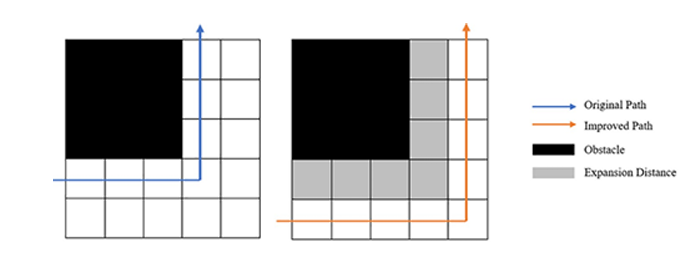
\includegraphics[ height=5cm]{p1}
		\caption{نمودار شماتیک فاصله توسعه}\label{p1}
    \end{figure}
    
\section{روش بهینه‌سازی جستجوی دوطرفه}\label{32}

الگوریتم \lr{A*} از شناخته‌شده‌ترین الگوریتم‌های برنامه‌ریزی مسیر است که برای یافتن کوتاه‌ترین مسیر بین نقطه شروع و هدف در گراف‌ها استفاده می‌شود. یکی از مشکلات اصلی این الگوریتم، پیچیدگی محاسباتی زیاد در گراف‌های بزرگ و پیچیده است که باعث افزایش زمان جستجو می‌شود.

برای رفع این مشکل، روش بهینه‌سازی جستجوی دوطرفه معرفی شده است. در این روش، جستجو همزمان از هر دو سمت گره شروع و گره هدف انجام می‌شود و مسیرهای جستجو به سمت یکدیگر پیش می‌روند تا در میانه راه به هم برسند و مسیر کامل ساخته شود. این کار باعث کاهش فضای جستجو و کاهش تعداد گره‌های مورد بررسی می‌شود و به طبع آن سرعت اجرای الگوریتم افزایش می‌یابد.

جستجوی دوطرفه بر اساس ارزیابی تابع هزینه کلی که در رابطه   \eqref{eq1} نشان داده شده است، انجام می‌شود. هر گره به عنوان گره بعدی که کمترین مقدار \( f(n) \) را دارد انتخاب می‌شود، ولی این انتخاب به صورت همزمان از دو طرف انجام می‌شود.

همچنین با استفاده از این روش، فضای جستجو کاهش یافته و تعداد فراخوانی‌های تابع به طور چشمگیری کمتر خواهد شد، خصوصاً در گراف‌های بسیار بزرگ که جستجوی یک‌طرفه زمان زیادی می‌برد.

شکل \ref{p2} نمونه‌هایی از بهینه‌سازی جستجوی دوطرفه را در گراف‌های مختلف نشان می‌دهد که چگونه جستجو از دو سمت باعث کاهش فضای جستجو و افزایش سرعت پیدا کردن مسیر می‌شود.
	\begin{figure}[H]
	\centering
	\begin{subfigure}{0.48\linewidth}
		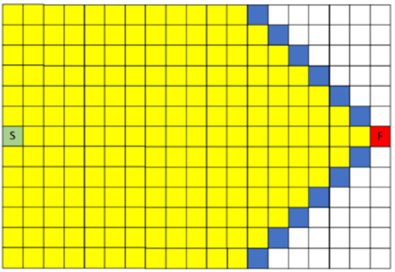
\includegraphics[width=\linewidth]{a}
		\subcaption{نمودار شماتیک جستجوی یک‌طرفه}\label{a}
	\end{subfigure}
	\begin{subfigure}{0.48\textwidth}
		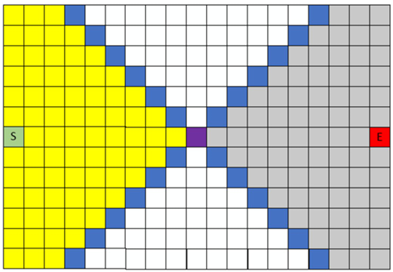
\includegraphics[width=\linewidth]{b}
		\subcaption{جستجوی دوطرفه بدون مانع}\label{b}
	\end{subfigure}
	\begin{subfigure}{0.48\textwidth}
	    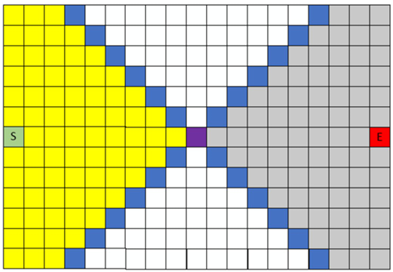
\includegraphics[width=\linewidth]{b}
	    \subcaption{جستجوی دوطرفه با یک مانع}\label{c}
    \end{subfigure}	
	\begin{subfigure}{0.48\textwidth}
	    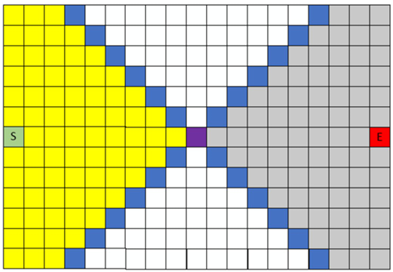
\includegraphics[width=\linewidth]{b}
	    \subcaption{جستجوی دوطرفه با موانع متعدد}\label{d}
    \end{subfigure}	
    \caption{نمودارهای شماتیک جستجوی دوطرفه}
    \label{p2}
\end{figure}


همان‌طور که در شکل \ref{p2} مشاهده می‌شود، جستجوی دوطرفه می‌تواند در شرایط مختلف عملکرد متفاوتی داشته باشد. در زیرشکل \ref{a}، جستجوی یک‌طرفه نشان داده شده است که در آن مسیر فقط از مبدأ به سمت هدف گسترش می‌یابد. در مقابل، زیرشکل‌های \subref{b} و \subref{c} و \subref{d} از شکل \ref{p2} به ترتیب جستجوی دوطرفه را در حالت بدون مانع، با یک مانع و با موانع متعدد نمایش می‌دهند. این مقایسه نشان می‌دهد که جستجوی دوطرفه با کاهش فضای جستجو، به ویژه در حضور موانع، کارایی بالاتری نسبت به حالت یک‌طرفه دارد.

\section{روش بهینه‌سازی هموارسازی مسیر}\label{33}

مسیر تولیدشده توسط الگوریتم \lr{A*} شامل قطعات خطی به هم پیوسته است که سه ایراد عمده دارد:

\begin{itemize}
	\item مسیر نهایی ناهموار است و زاویه‌های تند (عموماً 90 درجه) در آن وجود دارد.
	\item مسیر تولیدشده پیوسته نیست.
	\item وجود زاویه‌های تند منجر به کاهش سرعت حرکت ربات در آن نقاط می‌شود که باعث کاهش کارایی کل مسیر می‌گردد.
\end{itemize}

برای رفع این مشکلات، از روش هموارسازی مسیر استفاده می‌شود که در آن مسیر اصلی با یک منحنی نرم جایگزین می‌شود. یکی از بهترین روش‌ها برای این کار، استفاده از منحنی بزیه\LTRfootnote{\lr{Bezier Curve}} است.

منحنی بزیه دارای ویژگی‌های ریاضی مهمی است که از جمله مهمترین آنها خاصیت بازگشتی ضرایب برنشتاین\LTRfootnote{\lr{Bernstein}} می‌باشد. بر اساس این ویژگی، ضرایب منحنی بزیه از رابطه بازگشتی \eqref{eq3} پیروی می‌کنند که محاسبه نقاط روی منحنی را بدون نیاز به محاسبه مستقیم ضرایب دوجمله‌ای امکان‌پذیر می‌سازد.
\begin{align}
	B_{i,n}(t) &= (1 - t)B_{i,n-1}(t) + tB_{i-1,n-1}(t) \nonumber \\
	&= (1 - t)\left[(1 - t)B_{i,n-2}(t) + tB_{i-1,n-2}(t)\right] + t\left[(1 - t)B_{i-1,n-2}(t) + tB_{i-2,n-2}(t)\right] \nonumber \\
	&= (1 - t)^2 B_{i,n-2}(t) + 2t(1 - t)B_{i-1,n-2}(t) + t^2 B_{i-2,n-2}(t) \nonumber \\
	&= \sum_{k=0}^{m} \binom{m}{k} t^k (1 - t)^{m-k} B_{i-k, n-m}(t), \quad m \le i \le n
	\label{eq3}
\end{align}

بر اساس تعریف چندجمله‌ای‌های برنشتاین، منحنی بزیه از درجه \( n \) به صورت پارامتری و با ترکیب این چندجمله‌ای‌ها تعریف می‌شود. رابطه \eqref{eq4} نمایش کلی یک منحنی بزیه را بر حسب نقاط کنترل و چندجمله‌ای‌های پایه نشان می‌دهد.
\begin{equation}
	\mathrm{P}(t) = \sum_{i=1}^{n} p_i B_{i,n}(t), \quad t \in [0, 1]
	\label{eq4}
\end{equation}

در این رابطه، \( P_i(x_i, y_i)^T \) بردار مختصات \( i \)-امین نقطه کنترل و \( B_{i,n}(t) \) چندجمله‌ای پایه برنشتاین است که به صورت زیر تعریف می‌شود:
\begin{equation}
	B_{i,n}(t) = \binom{n}{i} t^i (1 - t)^{n-i}, \quad i = 0, 1, \dots, n
	\label{eq:bernstein}
\end{equation}

یکی از دلایل اصلی محبوبیت منحنی بزیه در مسائل برنامه‌ریزی مسیر، مشتق‌پذیری پیوسته آن است. مشتق مرتبه اول این منحنی بر حسب نقاط کنترل به صورت رابطه \eqref{eq5} قابل محاسبه می‌باشد که برای تعیین جهت حرکت ربات در طول مسیر کاربرد دارد.

\begin{equation}
	\dot{\mathrm{P}}(t) = \frac{d\mathrm{P}(t)}{dt} = n \sum_{i=0}^{n-1} B_{i,n-1}(t) (\mathrm{P}_{i+1} - \mathrm{P}_i)
	\label{eq5}
\end{equation}

به این ترتیب، با استفاده از منحنی بزیه می‌توان یک مسیر هموار با انحنای پیوسته ایجاد کرد که برای حرکت ربات‌های خودران بسیار مناسب است.

استراتژی اصلی بهبود مسیر، تقسیم گردش‌های تند 90 درجه به دو گردش مالیم‌تر 45 درجه است تا مسیر نرم‌تر و پیوسته شود و سرعت حرکت ربات حفظ گردد.
هنگامی که گردش‌های متوالی 90 درجه وجود داشته باشد، می‌توان نقطه شکست را حذف کرد و دو گره مجاور آن را مستقیماً به یکدیگر متصل نمود تا چندین گردش قائمه به تعداد کمی گردش حاد 45درجه تبدیل شوند، همانطور که در شکل \ref{smoothing} نشان داده شده است.

\begin{figure}[H]
	\centering
	\begin{subfigure}{0.48\linewidth}
		\centering
		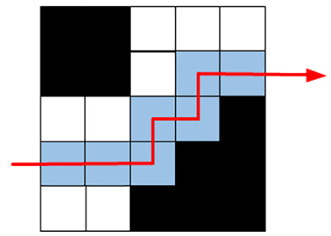
\includegraphics[width=\linewidth]{90}
		\subcaption{گردش 90 درجه}
		\label{90}
	\end{subfigure}
	%\hfill
	\begin{subfigure}{0.48\linewidth}
		\centering
		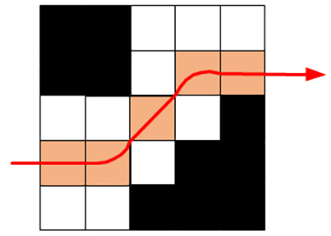
\includegraphics[width=\linewidth]{45}
		\subcaption{گردش 45 درجه پس از بهینه‌سازی}
		\label{45}
	\end{subfigure}
	\caption{استراتژی بهینه‌سازی هموارسازی برای گردش‌های متوالی قائم}
	\label{smoothing}
\end{figure}

در زیرشکل \subref{90} یک گردش 90 درجه مشاهده می‌شود که دارای زاویه تند و ناهموار است. پس از اعمال روش هموارسازی، این گردش به دو گردش 45 درجه در زیرشکل \subref{45} تبدیل می‌شود که مسیر نرم‌تر و پیوسته‌تری را ارائه می‌دهد.
\section{الگوریتم \lr{EBS-A*}}\label{34}
\subsection{روند اجرای الگوریتم}\label{341}
شبه‌کد الگوریتم \lr{EBS-A*} در زیر آورده شده است.

\begin{latin}
	\begin{algorithm}
		\caption{EBS-A* Algorithm}
		\label{ebs}
		\begin{algorithmic}[1]
			\Require Start node $Start_i$, goal node $End_i$, environment map $Map$, estimated cost $f(n)$
			\Ensure Path $PATH$
			
			\State Initialize $Map$, $PATH\_S$, $PATH\_E$
			\State Call $ExpansionDistance(1)$
			\State Create forward open list $OPEN\_LIST\_1$ and forward close list $CLOSE\_LIST\_1$
			\State Create backward open list $OPEN\_LIST\_2$ and backward close list $CLOSE\_LIST\_2$
			\State Add $Start_i$ to $OPEN\_LIST\_1$ and $End_i$ to $OPEN\_LIST\_2$
			
			\Repeat
			\State $node\_s \gets OPEN\_LIST\_1.removeNext()$
			\State $PATH\_S.add(node\_s)$
			\State $search(node\_s, OPEN\_LIST\_1, CLOSE\_LIST\_1)$
			\State $CLOSE\_LIST\_1.add(node\_s)$
			
			\State $node\_e \gets OPEN\_LIST\_2.removeNext()$
			\State $PATH\_E.add(node\_e)$
			\State $search(node\_e, OPEN\_LIST\_2, CLOSE\_LIST\_2)$
			\State $CLOSE\_LIST\_2.add(node\_e)$
			
			\Until{$node\_s = End_i$ or $node\_e = Start_i$ or $OPEN\_LIST\_1 = \emptyset$ or $OPEN\_LIST\_2 = \emptyset$ or $GetNeighbor(node\_s) \cap GetNeighbor(node\_e) \neq \emptyset$}
			
			\State $PATH \gets PATH\_S + reverse(PATH\_E)$
			\State $smooth(PATH)$
			\State \Return $PATH$
		\end{algorithmic}
	\end{algorithm}
\end{latin}
فرآیند اجرایی الگوریتم \lr{EBS-A*} شامل چهار مرحله است: 
\begin{enumerate}
	\item انجام بهینه‌سازی فاصله توسعه روی الگوریتم \lr{A*}.
	\item انجام جستجوی دوطرفه روی الگوریتم.
	\item تولید مسیر نامنعطف (ناهموار).
	\item انجام فرآیند هموارسازی برای تولید مسیر هموار.
\end{enumerate}


فرآیند اجرایی الگوریتم پیشنهادی در شکل \ref{ebsastar} نشان داده شده است.

\subsection{تحلیل پیچیدگی زمانی الگوریتم \lr{EBS-A*}}\label{342}
در این بخش، با ترکیب جستجوی دوطرفه و بهینه‌سازی هموارسازی گردش‌های قائمه، شبه‌کد الگوریتم \lr{EBS-A*} به صورت زیر ارائه می‌شود. این الگوریتم از یک حلقه دوگانه استفاده می‌کند. حلقه داخلی، گره‌های مجاور را در چهار جهت پیمایش کرده و گره با کمترین هزینه مشخص شده و به جدول باز اضافه می‌شود. حلقه خارجی، گره‌های جدول باز را تا پایان پیمایش صف، طی می‌کند. عوامل متعددی مانند مقیاس نقشه، موقعیت گره شروع و گره هدف، تأثیر آشکاری بر پیچیدگی زمانی الگوریتم‌های مختلف برنامه‌ریزی مسیر دارند. به طور کلی، پیچیدگی زمانی الگوریتم‌های مختلف به صورت زیر بیان می‌شود:

\begin{equation}
	T \in [\mathrm{O}(\min[m, n]), \mathrm{O}(m \times n)]
	\label{eq:time_complexity}
\end{equation}

در رابطه \eqref{eq:time_complexity}، \( m \) و \( n \) به ترتیب طول و عرض نقشه هستند. از آنجا که جستجوی دوطرفه یک استراتژی جستجو در دو جهت است، هنگامی که مسیر شدنی باشد، مسیر تشکیل‌شده در هر جهت جستجو از کل مسیر کوچک‌تر است که این امر تعداد گره‌های اضافه‌شده به جدول باز و تعداد دفعات پیمایش حلقه را کاهش می‌دهد. بنابراین، پیچیدگی زمانی الگوریتم \lr{EBS-A*} کمتر از یا مساوی نصف پیچیدگی زمانی الگوریتم سنتی \lr{A*} است.
\begin{figure}[H]

\begin{tikzpicture}[
	node distance=1.5cm,
	box/.style={rectangle, draw, rounded corners, minimum width=3cm, minimum height=1.6cm, align=center, font=\sffamily},
	arrow/.style={->, >=Implies, thick, double distance=2pt},
	singlearrow/.style={->, >=stealth, thick, dashed}
	]

	
	\node (astar) [box] {A*};
	\node (exp) [box, right of=astar, xshift=3cm] {Expansion\\distance};
	\node (bidir) [box, right of=exp, xshift=3cm] {Bidirectional\\search};
	\node (smooth) [box, right of=bidir, xshift=3cm] {Smoothing};
	
	\draw[arrow] (astar) -- (exp);
	\draw[arrow] (exp) -- (bidir);
	\draw[arrow] (bidir) -- (smooth);
	
	\node[below of=exp, yshift=-0.9cm, font=\small\sffamily] (planned) {planned path generation};
	\node[below of=smooth, yshift=-0.9cm, font=\small\sffamily] (smoothgen) {smooth path generation};
	
	\draw[singlearrow] (exp.south) -- (planned.north);
	\draw[singlearrow] (smooth.south) -- (smoothgen.north);
	
\end{tikzpicture}
	\caption{مراحل اجرای الگوریتم \lr{EBS-A*}}
	\label{ebsastar}
\end{figure}


